\documentclass{protokol}
\usepackage{graphicx}
\usepackage{float}

\usepackage{tikz}
\usetikzlibrary{calc}
\usetikzlibrary{arrows}


%====== Units =====
\usepackage{amssymb}
\usepackage{siunitx}
\sisetup{inter-unit-product =\ensuremath{\cdot}}
\sisetup{group-digits = integer}
\sisetup{output-decimal-marker = {,}}
\sisetup{exponent-product = \ensuremath{\cdot}}
\sisetup{separate-uncertainty}
\sisetup{tight-spacing = false}
%\sisetup{scientific-notation = true}
%\sisetup{round-mode=places,round-precision=4}
%\sisetup{evaluate-expression}


%====== Grafy =====
\usepackage{pgfplots}
\pgfplotsset{width=0.8\linewidth, compat=1.17}
\def\plotcscale{0.8}
\usepackage{pgfplotstable}
\usepackage[figurename=Obr.]{caption} % figure caption rename

\usepackage[siunitx]{circuitikz} % obvody
% \ctikzset{bipoles/length=1cm}

%====== Rovnice align block ======
\usepackage{amsmath}
\setlength{\jot}{10pt} % rozestup mezi řádky

\graphicspath{ {./img/} }

%====== Code blocks ======
\usepackage{listings}

\usepackage[most]{tcolorbox}
\newtcbox{\inlinecode}{on line, boxsep=0pt, left=2pt, right=2pt, top=2pt, bottom=2pt, colframe=gray, boxrule=0.5pt, arc=1pt, auto outer arc, before upper={\vphantom{dlg}}, tcbox raise base} % vytvoření inline boxu pro kód

\lstdefinelanguage{Spice}{
    alsoletter={.},  % Přidává tečku jako součást slov
    morekeywords={.lib, .STEP, .param, .MEAS, FIND, WHEN, END, VALUE, R, C, L, K, .SUBCKT, .ENDS, .MODEL, .INCLUDE, .AC, .DC, .TRAN, .PRINT, .PLOT, .PROBE, .WIDTH, .OPTIONS, .NODESET, .IC},
    keywordstyle=\color{blue}\bfseries,
    sensitive=false, % klíčová slova nejsou citlivá na velikost písmen
    morecomment=[l]{;}, % komentáře začínají hvězdičkou
    morestring=[b]", % řetězce uzavřené do uvozovek
}

\lstset{
  language=Spice,
  basicstyle=\ttfamily\small,
  breaklines=true,
  numbers=left,
  numberstyle=\tiny\color{gray},
  frame=single,
  rulecolor=\color{black},
  title=\lstname,
  keywordstyle=\color{blue}\bfseries,
  commentstyle=\color{green},
  stringstyle=\color{red},
  showstringspaces=false
}

%====== Vyplňte údaje ======
\jmeno{Tomáš Vavrinec}
\kod{240893}
\rocnik{}
\obor{MET}
\skupina{}
\spolupracoval{--}

\merenodne{--}
\odevzdanodne{--}
\nazev{4. Dvoustupňový zesilovač}
\cislo{4} %měřené úlohy

\predmet{Návrh analogových integrovaných obvodů}
\ustav{Ústav mikroelektroniky}
\skola{FEKT VUT v~Brně}

\def\para{x+0}
\def\parb{\para-80}


%citace 
\usepackage[backend=biber, style=iso-numeric, sortlocale=cs_CZ, autolang=other, language=czech]{biblatex}
\addbibresource{bibliography.bib}
\DeclareFieldFormat{labelnumberwidth}{\mkbibbrackets{#1}}
% hyperlinky
\usepackage[colorlinks]{hyperref}

% odstavce
\usepackage{parskip}

% Bloky kódu
\usepackage{xcolor}

%New colors defined below
\definecolor{codegreen}{rgb}{0,0.6,0}
\definecolor{codegray}{rgb}{0.5,0.5,0.5}
\definecolor{codepurple}{rgb}{0.58,0,0.82}
\definecolor{backcolour}{rgb}{0.95,0.95,0.92}

\usepackage{listings}
\lstdefinestyle{mystyle}{
  backgroundcolor=\color{backcolour}, commentstyle=\color{codegreen},
  keywordstyle=\color{magenta},
  numberstyle=\tiny\color{codegray},
  stringstyle=\color{codepurple},
  basicstyle=\ttfamily\footnotesize,
  breakatwhitespace=false,         
  breaklines=true,                 
  captionpos=b,                    
  keepspaces=true,                 
  numbers=left,                    
  numbersep=5pt,                  
  showspaces=false,                
  showstringspaces=false,
  showtabs=false,                  
  tabsize=2
}
\lstset{
	inputencoding=utf8,
	extendedchars=true,
	literate={á}{{\'a}}1 {č}{{\v{c}}}1 {ď}{{\v{d}}}1 {é}{{\'e}}1 {ě}{{\v{e}}}1 
           {í}{{\'i}}1 {ň}{{\v{n}}}1 {ó}{{\'o}}1 {ř}{{\v{r}}}1 {š}{{\v{s}}}1 
           {ť}{{\v{t}}}1 {ú}{{\'u}}1 {ů}{{\r{u}}}1 {ý}{{\'y}}1 {ž}{{\v{z}}}1 
           {Á}{{\'A}}1 {Č}{{\v{C}}}1 {Ď}{{\v{D}}}1 {É}{{\'E}}1 {Ě}{{\v{E}}}1 
           {Í}{{\'I}}1 {Ň}{{\v{N}}}1 {Ó}{{\'O}}1 {Ř}{{\v{R}}}1 {Š}{{\v{S}}}1 
           {Ť}{{\v{T}}}1 {Ú}{{\'U}}1 {Ů}{{\r{U}}}1 {Ý}{{\'Y}}1 {Ž}{{\v{Z}}}1,
	style=mystyle
	}

% Číslování
\pagenumbering{arabic}



% =========================================
% =============== DOKUMENT ================
% =========================================
\begin{document}
	%====== Vygenerování tabulky ======
	\maketitle

\section*{ZADÁNÍ ÚLOHY}
  Detailní popis jednotlivých úloh s návodem najdete v NAO\_PC.pdf, který je dostupný v E-learningu.

\begin{itemize}
    \item {\bf Simulací získejte hodnoty prahového napětí \(U_{TH0}\) pro dvě různé řady rozměrů tranzistorů.}
    \begin{itemize}
        \item konstantní poměr \(W/L = 5, kdy \$L\$ = 0.18; 0.3; 0.5; 0.8; 1; 2; 3; 5; 10\),
        \item různé rozměry: \(W/L = 0.22/0.18; 1/0.5; 2/0.5; 2/1; 5/1; 5/2; 10/5; 10/10; 40/10\),
        \item výše uvedené dva body budou provedeny pro tranzistor NMOS i PMOS.
    \end{itemize}
    \item {\bf Závislost prahového napětí \(U_{TH}\) na \(U_{SB}/U_{BS}\) (bulk efekt) Simulací získejte hodnoty prahového napětí \(U_{TH}\) pro napětí \(U_{BS}\) (NMOS) resp. \(U_{SB}\) (PMOS) v rozsahu \(0 [V]\) až \(500 [mV]\) s krokem \(50 [mV]\).}
    \item {\bf Závislost parametru modulace délky kanálu (\(\lambda\)) na délce kanálu (L) Simulací získejte hodnoty parametru \(\lambda\) tranzistoru NMOS a PMOS pro L v rozmezí \(200 [nm]\) až \(10 [\mu m]\).}
\end{itemize}

\subsection*{Bonusové otázky (1 b.)}
\begin{itemize}
    \item Popište, jak byste simulací (mimo analýzu \inlinecode{.op}) zjistili transkonduktanci \(gm\).
          Nakreslete schéma, popište nastavení a odečet hodnot.
\end{itemize}

\setcounter{section}{0}

\newpage
\section{Vypracování}
  \subsection{Zesilovač s odporovou zátěží} 
  Jako první určíme proud \(I_d\), to uděláme dvěma způsoby, podle požadovaného \(SR\) a podle požadovaného \(GBW\) a vybereme ten větší.

Podle \(SR\)
\begin{center}
    \large
    \(
        I_d = SR \cdot C_L = 10 \cdot 10^{6} \cdot 10 \cdot 10^{-12} = 100 [\mu A]
    \)
\end{center}

Podle \(GBW\) 
\begin{center}
    \large
    \(
        I_d = GBW \cdot U_{OV} \cdot \pi \cdot C_L = 10 \cdot 10^{6} \cdot 0.2 \cdot \pi \cdot 10\cdot 10^{-12} =  62.8 [\mu A]
    \)
\end{center}

Proud tedy bude \(I_{dM6} = 100 [\mu A]\) 

Dále můžeme určit rozměry tranzistorů \(M_6\) a \(M_7\), k čemuž budeme muset zvolit napětí \(U_{OV}\), která sme s ohledem na pracovní rozsah už v minulém kroku zvolili jako\(U_{OV} = 0.2 [V]\).
Délku tranzistoru \(L\) zvolím s ohledem na parametr \(\lambda\) \(L = 2 [\mu m]\).

\begin{center}
    \large
    \(
        W_{M6} = L \cdot \frac{2 \cdot I_d}{KP_N \cdot U_{OV}^2} = 2\mu \cdot \frac{2 \cdot 100\mu}{200\mu 0.2^2} = 50 [\mu m]
    \)
\end{center}

\begin{center}
    \large
    \(
        W_{M7} = L \cdot \frac{2 \cdot I_d}{KP_P \cdot U_{OV}^2} = 2\mu \cdot \frac{2 \cdot 100\mu}{50\mu 0.2^2} = 200 [\mu m]
    \)
\end{center}

Dále můžeme určit proud diferenčním stupněm jako desetinu destinu proudu výstupním stupněm, tedy \(I_{dM} = 10 [\mu A]\) z čehož můžeme určit rozměry tranzistorů \(M1\) až \(M_5\)

\begin{center}
    \large
    \(
        W_{M1,2} = L \cdot \frac{2 \cdot I_d}{KP_N \cdot U_{OV}^2} = 2\mu \cdot \frac{2 \cdot 10\mu}{200\mu 0.2^2} = 5 [\mu m]
    \)
\end{center}

\begin{center}
    \large
    \(
        W_{M4,5} = L \cdot \frac{2 \cdot I_d}{KP_P \cdot U_{OV}^2} = 2\mu \cdot \frac{2 \cdot 10\mu}{50\mu 0.2^2} = 20 [\mu m]
    \)
\end{center}

Proud tranzistorem \(M_3\) je součtem proudu \(I_{dM1}\) a \(I_{dM2}\) a tedy \(I_{dM3} = 20 [\mu A]\) jeho šířka tedy bude dvojnásobná \(W_{M3} = 10 [\mu A]\)
Tranzistor \(M_8\) zvolíme stejný jako tranzistor \(M_3\), tedy \(L=2 [\mu m] W=10[\mu m]\) a zbývá určit jen rezistor \(R_1\) jako:

\begin{center}
    \Large
    \(
        R_1 = \frac{U_{CC}-(U_{OV}+U_{TH})}{I_{dM3}} = \frac{1.8 - (0.2+0.4)}{20 \cdot 10^{-6}} = 60 [k\Omega]
    \)
\end{center}

\vspace{10mm}
\begin{figure}[h!]
    \centering
    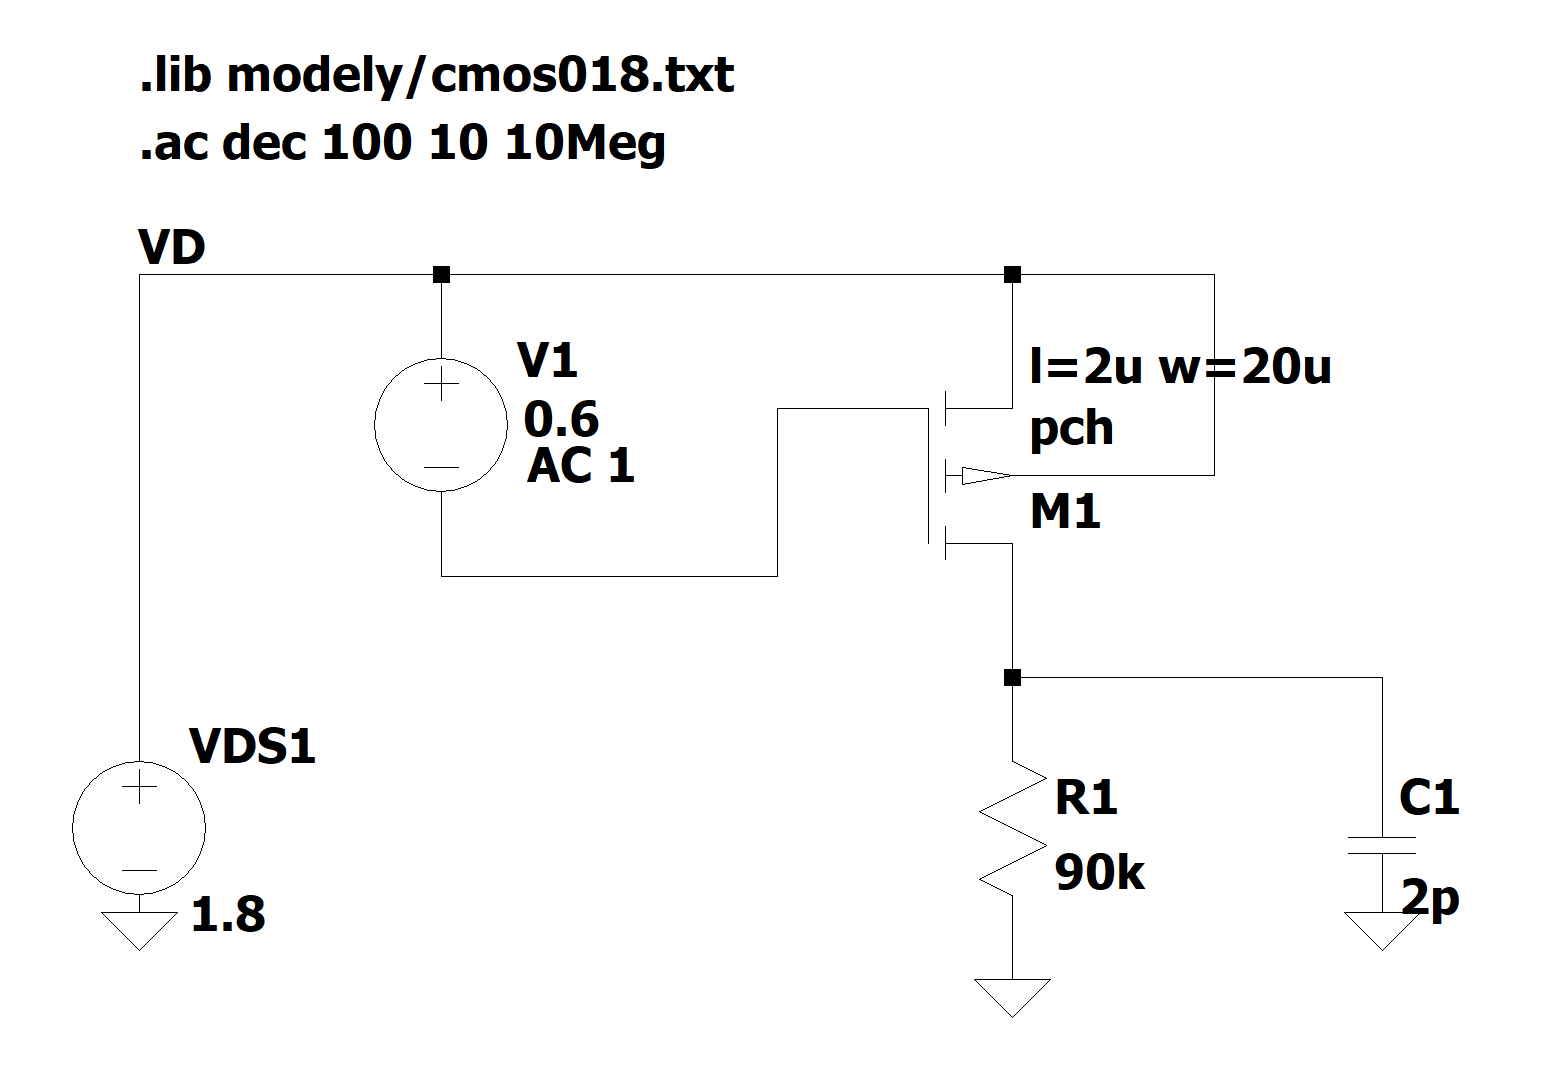
\includegraphics[width=0.6\textwidth]{text/img/Res-sch.png}
    \caption{\label{fig:res-sch} Schéma zesilovače}
\end{figure}

\vspace{10mm}
\begin{figure}[h!]
    \centering
    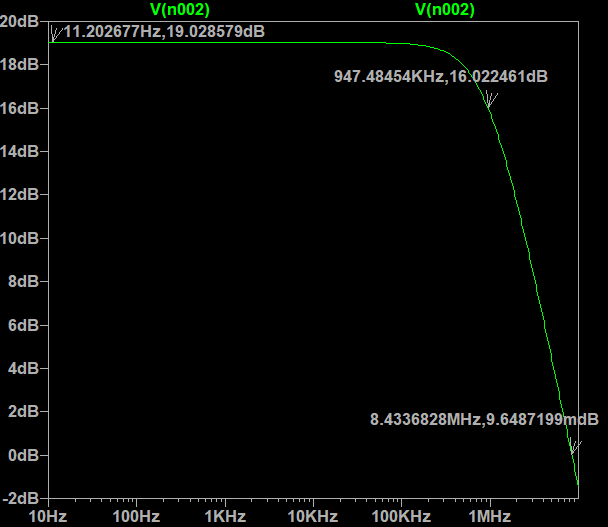
\includegraphics[width=0.8\textwidth]{text/img/Res-AC-graf.png}
    \caption{\label{fig:res-AC} {\bf .AC} analýza zesilovače}
\end{figure}
Zesílení mi vychází o necelý decibel menší než dle zadání, zkusil jsem tedy lehce zvětšit zatěžovací odpor na hodnotu \(R_1 = 102.48 [k\Omega]\) a obdržel jsem průběh \ref{fig:res-AC-102.48k}

\begin{figure}[h!]
    \centering
    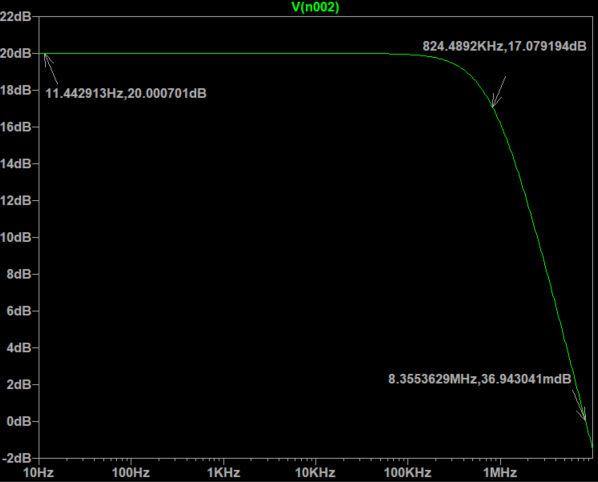
\includegraphics[width=0.8\textwidth]{text/img/Res-AC-graf-102.48k.png}
    \caption{\label{fig:res-AC-102.48k} {\bf .AC} analýza zesilovače se zvětšeným zatěžovacím odporem na \(R_1 = 102.48 [k\Omega]\)}
\end{figure}

\vspace{10mm}
\begin{figure}[h!]
    \centering
    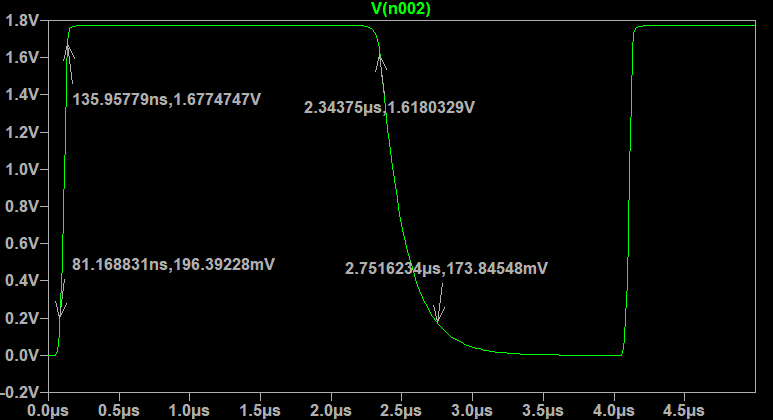
\includegraphics[width=0.9\textwidth]{text/img/Res-trans-graf.png}
    \caption{\label{fig:res-SR} {\bf .trans} analýza s vyznačenými body pro určení SR}
\end{figure}

Z průběhu \ref{fig:res-SR} určíme SR jako:
\begin{center}
    \Large
    \(
        SR_{rise} = \frac{\Delta U}{\Delta t} = \frac{U_2 - U_1}{t_2 - t_1} = \frac{1.677 - 0.196}{126n - 81n} = 32.9 [V/\mu s]
    \)

    \(
        SR_{fell} = \frac{\Delta U}{\Delta t} = \frac{U_1 - U_2}{t_2 - t_1} = \frac{1.618 - 0.174}{2752n - 2344n} = 3.5 [V/\mu s]
    \)
\end{center}

Sestupná hrana je pomalejší, než by dle zadání měla být, což je způsobeno předpokladem lineárního vybíjení kondenzátoru \(C_1\), zatím co je exponenciální, jak je vidět na průběhu \ref{fig:res-SR}

\(GBW\) je větší, než bylo požadováno, protože proud tranzistorem jsme stanovili vyšší, abychom splnili \(SR\).

  \newpage
  \clearpage

%   \subsection{Zesilovač s aktivní zátěží} 
%   Při návrhu aktivní zátěže, začneme návrhem rozměrů tranzistorů.
Délku kanálu \(L\) zvolíme opět \(L = 2 [\mu m]\) a napětí \(U_{TH} = 0.2 [V]\), šířku kanálu \(W\) pak určíme jako:

\begin{center}
    \large
    \(
        W_{M2} = W_{M3} = L \cdot \frac{2 \cdot I_d}{KP \cdot U_{OV}^2} = 2\mu \cdot \frac{2 \cdot 10\mu}{200\mu 0.2^2} = 5 [\mu m]
    \)
\end{center}

Následně určíme odpor nastavující proud tranzistorem \(M_3\) jako:

\begin{center}
    \large
    \(
        R_{1} = \frac{U_{CC} - (U_{TH} + U_{OV})}{I_D} = \frac{1.8-(0.4+0.2)}{10\mu} = 120 [k\Omega] 
    \)
\end{center}

\vspace{10mm}
\begin{figure}[h!]
    \centering
    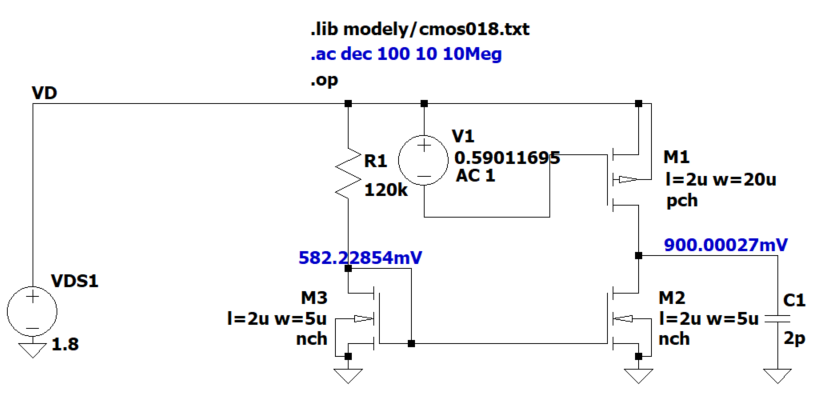
\includegraphics[width=0.8\textwidth]{text/img/Akt-sch.png}
    \caption{\label{fig:Akt-sch} Schéma zesilovače s aktivní zátěží}
\end{figure}

\vspace{10mm}
\begin{figure}[h!]
    \centering
    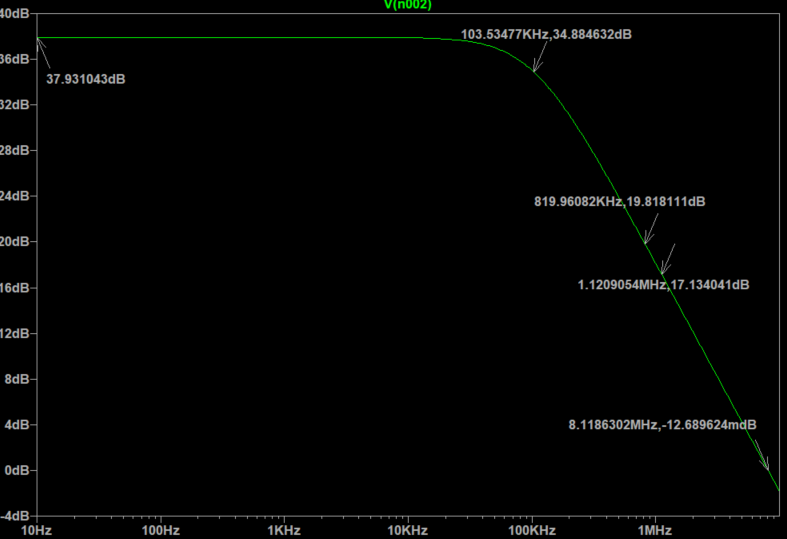
\includegraphics[width=0.7\textwidth]{text/img/Akt-AC-graf.png}
    \caption{\label{fig:Akt-AC} {\bf .AC} analýza zesilovače s aktivní zátěží}
\end{figure}

Zesílení s aktivní zátěží vychází o \(19 [dB]\) vyšší než v případě s odporovou zátěží.
Pokles o \(3 [dB]\) nastává mnohem dříve místo \(824 [kHz]\) už při \(104 [kHz]\).
Naproti tomu i při frekvenci \(824 [kHz]\) má zesilovač vyšší zesílení než případ z odporovou zátěží a ke stejnému zesílení, tedy \(17 [dB]\) dochází až u frekvence \(1.12 [MHz]\).
Zesilovač s aktivní zátěží má ale strmější pokles, protože přestává zesilovat na frekvenci \(GBW = 8.12 [MHz]\), zatím co odporová varianta zesiluje až do \(GBW = 8.43 [MHz]\).

\vspace{10mm}
\begin{figure}[h!]
    \centering
    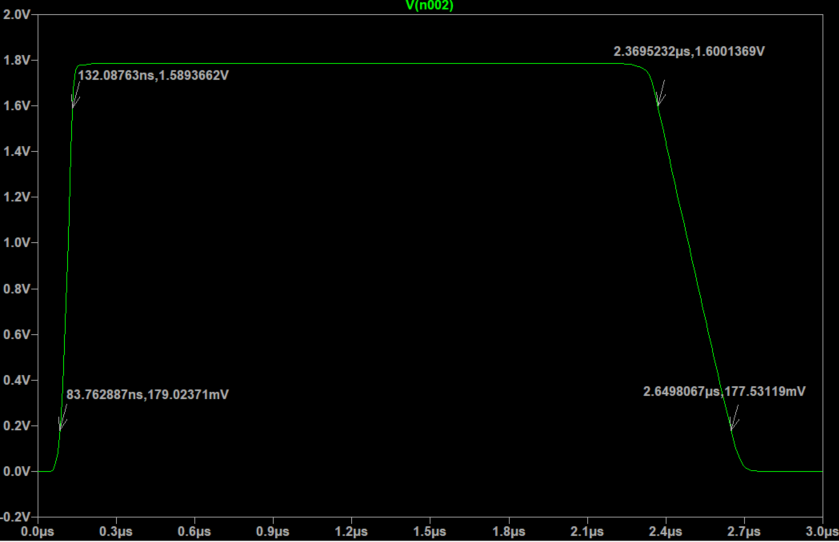
\includegraphics[width=0.7\textwidth]{text/img/Akt-trans-graf.png}
    \caption{\label{fig:res-SR} {\bf .trans} analýza s vyznačenými body pro určení SR}
\end{figure}

Z průběhu \ref{fig:res-SR} určíme SR jako:
\begin{center}
    \Large
    \(
        SR_{rise} = \frac{\Delta U}{\Delta t} = \frac{U_2 - U_1}{t_2 - t_1} = \frac{1.589 - 0.179}{132n - 87n} = 31.3 [V/\mu s]
    \)

    \(
        SR_{fell} = \frac{\Delta U}{\Delta t} = \frac{U_1 - U_2}{t_2 - t_1} = \frac{1.6 - 0.178}{2650n - 2367n} = 5 [V/\mu s]
    \)
\end{center}

Zde je vidět že sestupná hrana už zadání přesně splňuje.

%   % \newpage
%   % \clearpage
%   % \subsection{Napěťová reference s proudovým zdrojem} 
%   % V předchozím příkladě napěťové reference sloužil odpor \(r_1\) jako proudoví zdroj.
Protože jde jen o rezistor nebude to dvakrát přesný proudoví zdroj a proto ho nyní nahradíme proudovým zdrojem z předcházejícího příkladu.
Hodnoty všech prvku zůstávají zachovány a výsledkem je tedy následující schéma.

\begin{figure}[h!]
    \centering
    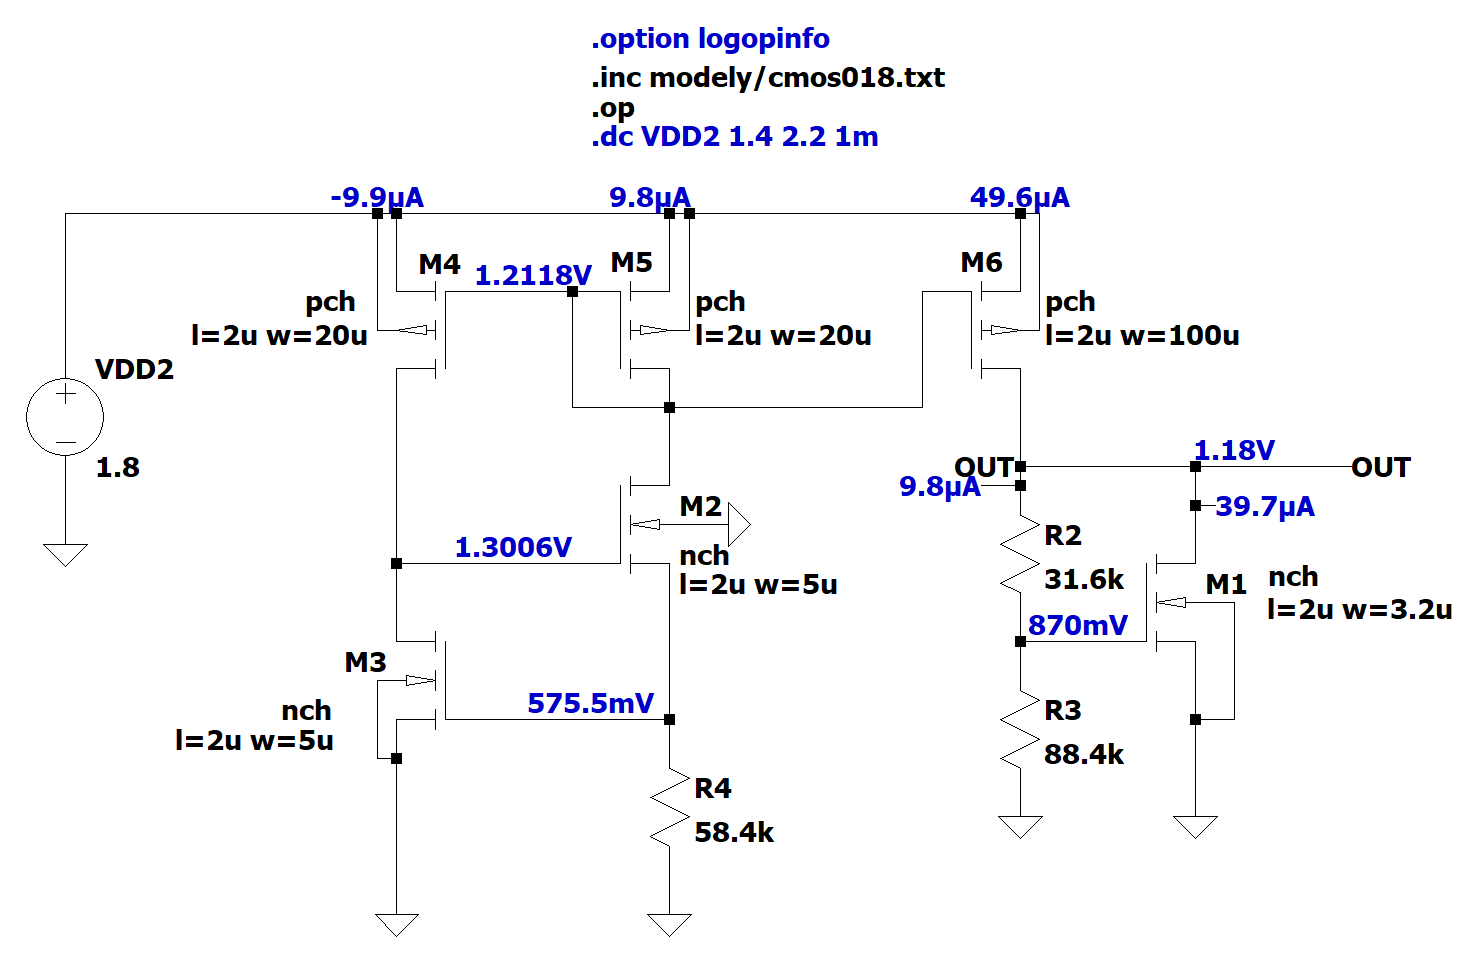
\includegraphics[width=0.9\textwidth]{text/img/LNR-op-sch.png}
    \caption{\label{fig:LNR-op-sch} Zobrazení napětí a proudu ve schématu}
\end{figure}

\vspace{10mm}
\begin{figure}[h!]
    \centering
    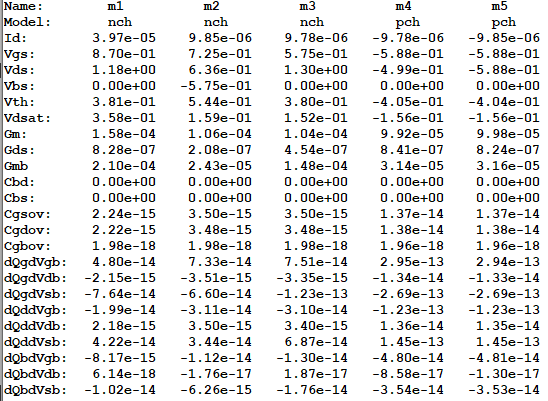
\includegraphics[width=0.9\textwidth]{text/img/LNR-op-ol.png}
    \caption{\label{fig:LNR-op-ol} Pracovní bod tranzistoru}
\end{figure}

\begin{figure}[h!]
    \centering
    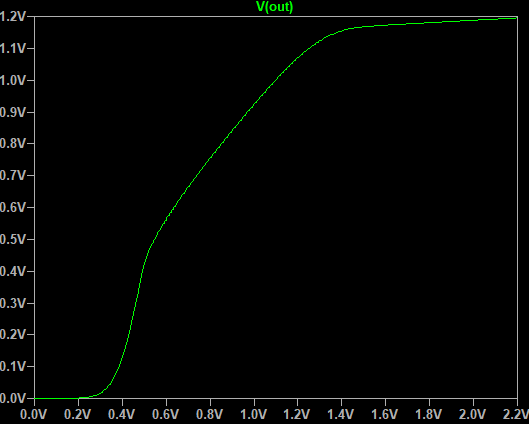
\includegraphics[width=0.9\textwidth]{text/img/LPR_zavislost.png}
    \caption{\label{fig:LNR-zav} Zobrazení napětí a proudu ve schématu}
\end{figure}

\vspace{10mm}
\begin{figure}[h!]
    \centering
    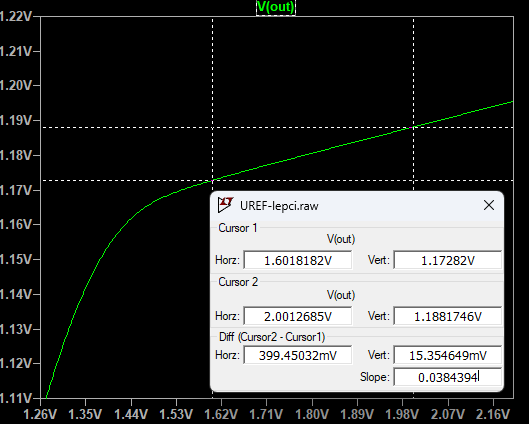
\includegraphics[width=0.9\textwidth]{text/img/LPR-detail_zavislosti.png}
    \caption{\label{fig:LNR-det-zav} Pracovní bod tranzistoru}
\end{figure}


%   % \newpage

\section{Závěr}
  Porovnání obou verzí zesilovače.

\begin{table}[h]
    \centering
    \begin{tabular}{|l|c|c|c|}
        \hline
        \textbf{Typ zátěže} & \textbf{Zesílení \(A_{U0} [-]\)} & \textbf{Rychlost přeběhu  \(SR_{fell} [V/\mu s]\)} & \textbf{šířka pásma \(GBW [MHz]\)} \\ \hline
        Odporová            & 19                               & 3.5                                                & 8.43                               \\ \hline
        Aktivní             & 38                               & 5.0                                                & 8.12                               \\ \hline
    \end{tabular}
    \caption{Porovnání obou typů zátěže}
    \label{tab:zrcadla}
\end{table}

% \clearpage
% \section*{Reference}
% \printbibliography[heading=none]

\end{document}